\chapter{Towards a Human Genome Variation Map}
\label{ch:hgvm}

\section{Introduction}

In Chapter~\ref{ch:bakeoff}, it was demonstrated that the use of graph-based genomic references can result in improved variant calling performance over traditional linear references. However, in that study, the graph references that produced the most accurate variant calls compared to truth VCFs were derived from the 1000 Genomes Project's main variant call files~\cite{10002015global}, and allowed the detection of only relatively short indels, under about 50~bp~(Fig.~\ref{fig:bakeoff:refnonref}~(C)). Compared to the approximate 300~bp length of a single Alu repeat insertion~\cite{weiner1980abundant}, this is inadequate.

In addition to comparison against traditional Illumina-based variant calls, variant call accuracy was also evaluated using PacBio-based assembly data, by measuring how well the sample graph produced from the variant calls for a pooled synthetic diploid sample agreed with separate haploid assemblies. By this metric, variant calling performed with Cactus-based graphs was found to be more accurate than variant calling performed with 1000 Genomes-derived graphs~(Fig.~\ref{fig:bakeoff:calling}~(B)). Cactus-based graphs were also shown to allow the detection of longer insertions and deletions than 1000 Genomes-based graphs can find~(Fig.~\ref{fig:bakeoff:refnonref}~(C)). Overall, Cactus-based graphs, which are produced from the alignment of long alternate loci sequences, have some important advantages that 1000 Genomes-based graphs lack.

In order to construct a versatile graph-based reference that will serve as a community resource for read mapping and variant calling, it is desirable to combine the best aspects of these two types of graph. Additionally, as the bake-off project of Chapter~\ref{ch:bakeoff} worked only on regions up to a few megabases in size, it is desirable to demonstrate the effectiveness of graph-based methods at larger scales, where qualities like the ability to resolve mappings between ambiguous regions, and the ability to effectively use paired-end information, are more critical.

In this chapter, we present a method to create graph references combining the best qualities of 1000 Genomes-based and Cactus-based graphs, and validate these graphs on the scale of a chromosome.

\section{Methods}

\subsection{Graph Construction}

In order to combine a Cactus-based graph with a 1000 Genomes-based graph, we implemented a new subcommand in the \vg variation graph toolkit~\cite{garrison2016vg}. The new tool, \texttt{vg add}, augments an existing graph by inserting variants from a VCF file. It works by extracting local haplotypes around each variant that are consistent with the phased samples in the VCF file, and then aligning them to the relevant region of the graph, as determined by tracing an embedded primary reference path in the graph. For particularly large insertions and deletions, where a complete local alignment would be impractical, the ends of the variant are aligned, and the resulting alignments are stitched together to describe the actual variant.

The \texttt{vg add} tool, along with a Toil-based orchestration script~\cite{vivian2017toil}, were used to combine variation information from three sources. The base level graph was obtained using Cactus~\cite{paten2011cactus2}, by aligning together the chromosome 22 primary sequence and the chromosome 22 alt loci and so-called \vocab{random sequences} (which are localized to a chromosome but not placed along it) from GRCh38. The alignment was performed such that the main chromosome 22 sequence and the random sequences were not aligned to themselves or each other; only the alt sequences were allowed to align to the other sequences.
% TODO: What patch level did Joel use?
The Cactus alignment was converted to a \vg graph with the \texttt{hal2vg} tool\footnote{\url{https://github.com/ComparativeGenomicsToolkit/hal2vg}}, and the resulting graph had its nodes chopped to a maximum length of 1000~bp using \texttt{vg mod}.

\begin{sloppypar}
On top of this graph, \texttt{vg add} was used to add in variants from the 1000 Genomes Phase 3 GRCh38 lifted-over VCF files\footnote{\url{ftp://ftp.1000genomes.ebi.ac.uk/vol1/ftp/release/20130502/supporting/GRCh38_positions/}}. Notably, these variant files as distributed by the 1000 Genomes Project are not valid; variants lifted over to the reverse strand of GRCh38 are marked as marked with a \texttt{MATCHED\_REV} tag in the \texttt{INFO} field but left in their GRCh37 orientations, and needed to be reverse-complemented using a script so that the \texttt{REF} field contents will match the actual reference sequence at the variant's location.
\end{sloppypar}

\begin{sloppypar}
% TODO: what source data and processing script did Charlie use?
The \texttt{vg add} tool was also used to add structural variants to the graph. Since the structural variants in GRCh38 coordinates as originally obtained\footnote{\url{ftp://ftp.1000genomes.ebi.ac.uk/vol1/ftp/phase3/integrated_sv_map/supporting/GRCh38_positions/}} were described using a complex combination of \texttt{INFO} tags, additional tables, and references to difficult-to-locate external sequence database records, the files had to be preprocessed in order for \texttt{vg add} to be able to parse them. All variant alt information was moved into a fully realized concrete sequence in each variant record's \texttt{ALT} column, and the reference sequences, even for very long deletions, were placed in each variant record's \texttt{REF} column. All symbolic allele references and target site duplication sequences were resolved. For mobile element insertions, the original VCF specified the presence, but not the exact length, of a poly-A tail; in these cases, several duplicate variant records were created, with poly-A tail lengths of 10, 25, and 50 bases. This approach was selected in hopes of providing a mapping target sufficient to collect reads showing the correct poly-A tail length, which could then potentially be determined through graph-based variant calling.
\end{sloppypar}

Once the graph was fully constructed, it was indexed using \vg. This produced the XG and GCSA2 indexes that were required to align reads to the graph. The graph was then subjected to two evaluations, based on aligning reads to and variant calling against it. The structural variant evaluation, described in Subsection~\ref{subsec:structuralvariantevaluation}, involved comparing variant calls against a truth set, while the assembly realignment evaluation, described in Subsection~\ref{subsec:assemblyrealignmentevaluation}, involved evaluating the sample graph derived from the variant calls with reference to a pair of haploid assemblies.

\subsection{Variant Calling Techniques}
\label{subsec:variantcalling}

Both of the evaluations presented here relied on some improvements to the \vg variant caller, \texttt{vg call}, made for the purpose of this study. Previously, the caller operated only on sites defined by top-level ultrabubbles~\cite{paten2017superbubbles}, and exclusively produced VCF output. However, when working with the very large top-level ultrabubbles induced by the inclusion of large structural variants in the graph, it became necessary to consider nesting of ultrabubbles. The core of the caller was rewritten to handle ultrabubbles recursively. In this method, each ultrabubble is treated as a site. Calls are made on each top-level site while abstracting away variation inside of nested child sites, and then each nested child site is recursed on and a call is made for it in accordance with the copy number assigned to it by the higher-level call. An attempt was made to patch the lower-level call results into the output for the higher-level containing sites, subject to the limitation that within alternate alleles each child was always represented by its highest-coverage traversal, even if it was given a heterozygous call. This limitation was added to avoid difficult situations related to phasing between adjacent heterozygous children.

Additionally, in order to allow ultrabubbles that were not traversed by a primary reference path to be usefully called, the caller was modified to be able to output its calls in \texttt{Locus} format, in addition to VCF. This format is a binary, Protobuf-based format, similar to the other formats used by \vg, and represents calls as \texttt{Locus} objects. A \texttt{Locus} can have a series of graph paths stored within it as alternative alleles, along with zero or more genotypes called as potentially-empty collections of the available alleles at the \texttt{Locus}. This format allowed for each top-level site to be represented, and also allowed for child sites to be represented. Additionally, it allowed gVCF-like assertions to be made about the existence of a primary reference path outside of variable sites, by creating \texttt{Locus} objects covering non-variable material.

To improve performance on calling large structural variants, and to account for the transition to a recursive, child-abstracting architecture, numerous changes to the internal heuristics used by the variant caller were made. These changes were made manually, working primarily on the NA12878 sample; no automatic optimization of caller parameters was performed. All variant calls created in this study were performed using the default \texttt{vg call} heuristic parameters and an additional \texttt{--max-dp-multiple 2.5} setting.

Since sample graphs were required for the assembly realignment evaluation, the \texttt{vg mod} tool that produces sample graphs was enhanced to allow it to read and process calls in \texttt{Locus} format. Sample graphs were produced for \texttt{Locus}-format calls by eliminating all nodes and edges not called as present in some \texttt{Locus}.

\subsection{Assembly Realignment Evaluation}
\label{subsec:assemblyrealignmentevaluation}

The first evaluation was a variant of the assembly realignment evaluation from Chapter~\ref{ch:bakeoff}. A synthetic diploid sample was created from the CHM1 and CHM13 hydatidiform mole samples aligned to GRCh38 (it was actually the same sample used in Chapter~\ref{ch:bakeoff}). From this sample, read pairs where either member mapped to chromosome~22 or any of its random or alt scaffolds were collected. 

These reads were aligned to the graph under test and used for variant calling against it. However, instead of calling variants to VCF, we used our improved version of \texttt{vg call} to produce \texttt{Locus}-format variant calls for the ultrabubbles in the augmented graph (including both parent and nested child ultrabubbles)~\cite{paten2017superbubbles}, and assertions of the presence of all primary reference path edges not involved in ultrabubbles. Finally, as in Chapter~\ref{ch:bakeoff}, the augmented graph was subsetted to create a sample graph. Each graph under test was also evaluated as if it were a sample graph, without the variant calling and subsetting steps, in order to provide a control.

We evaluated two graphs in this way: the ``HGVM'' graph, created using Cactus and \texttt{vg add}, as described above, and a ``Control'' graph, consisting of just the chromosome 22 GRCh38 scaffold and associated random scaffolds, with no variants added. Each of these gave rise to one actual sample graph, produced by the variant caller, and one control sample graph, produced by passing through the entire graph under test as if it were the sample graph.

To evaluate each sample graph, the scaffolds from the CHM1 and CHM13 assemblies relevant to chromosome 22 were determined using a script. This script aligned 10~kb chunks of each scaffold every 100,000~kb to the 24 primary GRCh38 chromosome scaffolds, until a hit scoring 95\% of the maximum possible score was obtained. All scaffolds for which that first sufficiently good hit was to chromosome 22 were taken and chopped into pieces every 1000~bp to produce a set of assembly fragments. (The exception was scaffold \texttt{LBHZ02000095.1} from CHM13, which was manually found to consist of sequence mapping primarily to chromosome 13, and consequently excluded.) Overall, the analysis used 37,931,872~bp of sequence from CHM1 and 36,306,973~bp of sequence from CHM13. The assembly fragments were realigned against each indexed sample graph, and the quality of each sample graph as a representation of the assembly fragments was then measured. This was accomplished by going over the alignments and tabulating the total number of inserted, deleted, substituted, and softclipped bases, and dividing that total by the size of the Control graph (which consisted of chromosome 22 and the associated random sequences), to get a number of affected bases per primary reference base in each category.

\subsection{Structural Variant Evaluation}
\label{subsec:structuralvariantevaluation}

The second evaluation, by contrast, was a truth set VCF-based measurement of the accuracy of structural variant calls. Reads aligned to GRCh38 were obtained for five samples: NA12878, NA12889, and NA12890 from the Illumina Platinum Genomes dataset, and HG00513 and HG00732 from the 1000 Genomes High Coverage dataset. From each file of aligned reads, read pairs where either member mapped to chromosome 22 or any of its random or alt scaffolds were collected. These reads were then mapped to the graph under test, and variant calling for each sample was performed. Variant calls in VCF format were obtained. For each sample, the called VCF was compared against the GRCh38 structural variant files that were used for preparing the graph. Recall was computed by considering each unique variant position in the truth VCF for which an alternate allele was called in the sample, and treating it as recalled if the variant calls for the sample in question contained a variant with a length change of 25~bp or more, having a position within 25~bp of the truth position. Filtered variants were ignored in both VCFs. Because the truth set VCF used was not believed or warranted to be complete, precision was computed manually, by randomly sampling a certain number of calls for variants with length changes of 25~bp or more with calls of alternate alleles, and manually classifying each selected positive call as true or false, by looking at the original input reads and the truth VCF at the variant's location on the UCSC genome browser.

\subsection{Software and Hardware}
\label{subsec:azurecluster}

\begin{sloppypar}
The graph construction and evaluation was performed on a Microsoft Azure cluster using five \texttt{Standard\_G5} worker nodes and one \texttt{Standard\_A5} master, managed using the Toil workflow engine~\cite{vivian2017toil}. The \path{quay.io/vgteam/vg:v1.5.0-303-gb1a6cc8c-t62-run} Docker container provided the \vg build used in this study.
\end{sloppypar}


\section{Results}

\subsection{Graph Construction}

The cluster run to build the graph, starting from the vg-format Cactus graph, and to run the structural variant and assembly realignment evaluations, took 20 hours, 16 minutes, and 35 seconds on the Microsoft Azure cluster described above in Subsection~\ref{subsec:azurecluster}. No attempt was made to fit the size or resource allocations of the cluster to the requirements of the workflow; the analysis succeeded on the smallest (and only) cluster on which it was tried.

The final chromosome 22 graph contained 3,630,637~nodes and 4,736,765~edges, with a total length (summed over all nodes) of 57,097,953~bp. The initial input data consisted of 51,857,516~bp of primary reference and random scaffold sequence, and 1,625,159~bp of alternate loci (much of which should have aligned to and been merged with the primary reference and random sequences), meaning that at least 3,615,278~bp of material, or 6.97\%, was created by \texttt{vg add} from VCF files. The input VCF files only had 132,693~bp of structural variant alternate allele sequence and and 1,167,426~bp of point variant alternate allele sequence. The graph was found to contain 3,750,000~bp of \texttt{N} bases not on any of the paths from the base Cactus graph. Extraneous \texttt{N} bases were observed occurring in large collections of parallel nodes containing mostly \texttt{N} bases. However, as extraneous runs of \texttt{N}s do not attract reads that ought to map elsewhere, the graph was still used for further alignment-based analyses.

The graph contained 10~``head'' nodes, with nothing attached to their left sides, and 10~``tail'' nodes, with nothing attached to their right sides. This was consistent with the 10~primary path sequences (\texttt{chr22} and 9~unlocalized chromosome 22 scaffolds) used to construct the base graph.

\subsection{Assembly Realignment Evaluation}
\label{subsec:assemblyrealignmenteval}

For the first evaluation, based on realignment of the mole reads, results are visible in Figure~\ref{fig:molerealignment}. Two graphs were used in the evaluation: the final chromosome 22 HGVM graph, and the Control graph constructed only from chromosome 22 and the associated random sequences in GRCh38, without any alignment or additional variants. Each of these graphs was used as a reference for read alignment and variant calling, and the resulting sample graphs are the ``HGVM'' and ``Control'' conditions in the figure. Each of the graphs was also evaluated as if it were a sample graph, producing the ``No Call'' and ``All Ref'' conditions, respectively.

On the Deletions, Insertions, and Substitutions metrics (although by a very small margin on the Insertions metric), the HGVM condition performed best. Calling variants based on the graph reference, with its included known variation, resulted in needing to delete fewer bases, insert fewer bases, and substitute fewer bases to explain the assembly fragment truth set, compared to when variant calling was done using the Control graph, which contained no embedded variation. Additionally, the variant calling step itself reduced the number of bases that needed to be deleted by a large factor, and the number of bases that needed to be inserted or substituted slightly, as can be seen by comparing the HGVM condition to the No Call condition (Fig.~\ref{fig:molerealignment}). This suggests that the variant caller is successful in incorporating information from aligned reads into the sample graph. Finally, note that, for deletions, substitutions, and insertions, the decrease in required base modifications attributable to the variant caller operating on the variation-containing graph (i.e. the drop from No Call to HGVM) was greater than the decrease attributable to the variant caller operating on the no-variation graph (i.e. the drop from All Ref to Control). This shows that including variation in the reference can make variant callers more effective.

On the softclips metric, on the other hand, the ``No Call'' condition outperformed the ``HGVM'' condition by a small margin, meaning that the graph reference with no variant call performed on it was a better match for the assembly fragments being realigned than was the sample graph produced by variant calling, in terms of the number of softclipped bases required in the assembly fragments' alignments.

\begin{FPfigure}
\centering
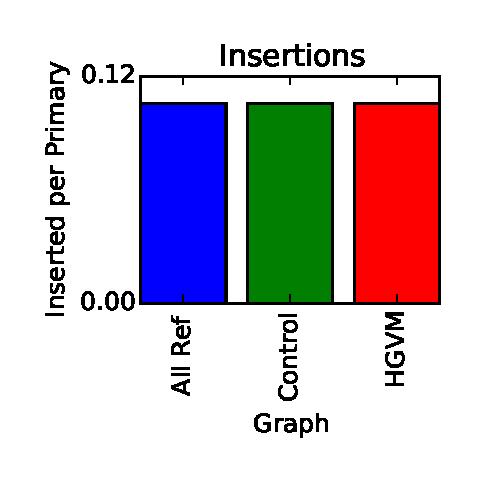
\includegraphics[width=0.4\linewidth]{figures/05_hgvm/mole-insertions.eps}
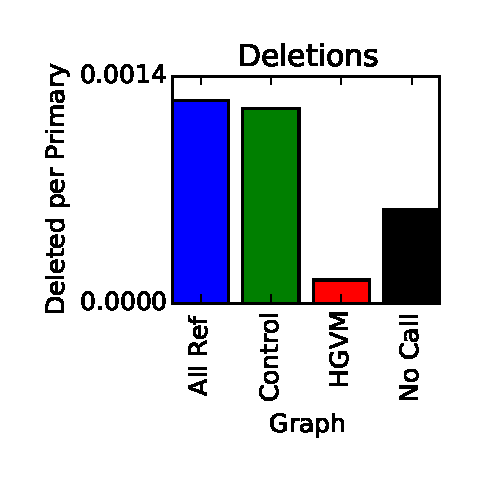
\includegraphics[width=0.4\linewidth]{figures/05_hgvm/mole-deletions.eps}
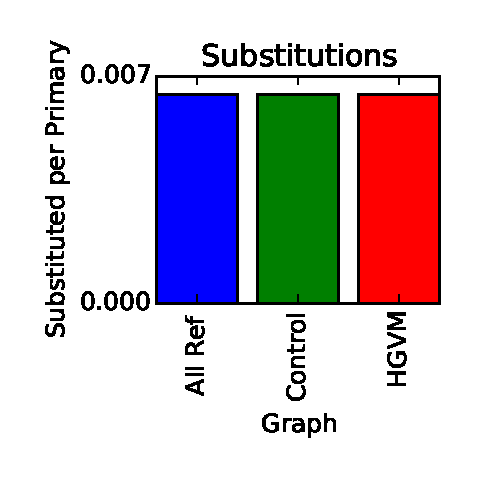
\includegraphics[width=0.4\linewidth]{figures/05_hgvm/mole-substitutions.eps}
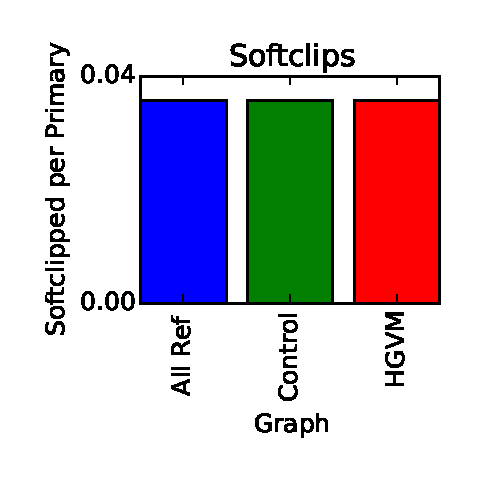
\includegraphics[width=0.4\linewidth]{figures/05_hgvm/mole-softclips.eps}
\caption[Mole realignment evaluation]{Bases involved in events required to align fragments of the CHM1 and CHM13 haploid assemblies to the sample graph created with the \vg variant caller for the combined synthetic diploid sample. Quantities are expressed as bases involved in each type of event per base in the control graph. For the All Ref condition (blue), the performance of the primary-reference-only control graph as a sample graph was evaluated. For the Control condition (green), that reference-only graph was used as a reference for variant calling, and the resulting sample graph was evaluated. For the HGVM condition (red), the Human Genome Variation Map graph under test was used as a reference for variant calling, and the resulting sample graph was evaluated. Finally, for the No Call condition (black), the HGVM graph was evaluated directly as a sample graph, with no calling step, to serve as a positive control.}
\label{fig:molerealignment}
\end{FPfigure}
% TODO: make a table of this?

\subsection{Structural Variant Evaluation}
\label{subsec:structuralvarianteval}

For the second, VCF-based evaluation, the precision statistics for the five samples analyzed (HG00513, HG00732, NA12878, NA12887, and NA12890) are visible in Table~\ref{tbl:svprecision}, while the recall results for the samples are visible in Table~\ref{tbl:svrecall}.
Summing across samples, the overall precision was~20~out of~25, or 0.80, while the overall recall was~106~of~151, or~0.702. Together, these produce an F1 score of 0.76.

\newcommand{\true}{\textbullet}
\newcommand{\false}{}

\begin{FPsidewaystable}
\centering
\begin{tabular} {l|c|c|r|c|c|c|c}
\textbf{Sample} & \textbf{Position} & \textbf{Type} & \textbf{Length (bp)} & \textbf{1KG SV Call} & \textbf{In dbSNP} & \textbf{In Reads} & \textbf{True} \\
\hline
HG00513 & 37661330 & Deletion & 28 & \false & \true & \true & \true \\
HG00513 & 44246856 & Insertion & 33 & \false & \true & \true & \true \\
HG00513 & 45210755 & Insertion & 36 & \false & \true & \true & \true \\
HG00513 & 49343564 & Deletion & 28 & \false & \true & \true & \true \\
HG00513 & 49354907 & Deletion & 57 & \true & \true & \true & \true \\ % The dbSNP variant here si slightly offset from where we want it to be

HG00732 & 23946708 & Insertion & 1164 & \false & \false & \true & \true \\
HG00732 & 22955032 & Deletion & 38 & \false & \false & \true & \true \\
HG00732 & 36731029 & Deletion & 172 & \true & \true & \true & \true \\
HG00732 & 39195778 & Deletion & 28 & \false & \true & \true & \true \\
HG00732 & 41552577 & Insertion & 40 & \false & \true & \true & \true \\

NA12878 & 17801142 & Deletion & 322 & \false & \false & \false & \false \\ % Other samples have this deletion called in the 1kg SVs but not NA12878
NA12878 & 24005821 & Deletion & 52 & \false & \false & \false & \false \\ % This is one of those 90 depth ones...
NA12878 & 25232595 & Deletion & 42 & \false & \true & \true & \true \\
NA12878 & 44246856 & Insertion & 33 & \false & \true & \true & \true \\
NA12878 & 47920718 & Deletion & 25 & \false & \true & \true & \true \\

NA12889 & 17717386 & Insertion & 33 & \false & \true & \true & \true \\
NA12887 & 20224942 & Insertion & 29 & \false & \true & \true & \true \\
NA12887 & 23506174 & Insertion & 1095 & \false & \false & \false & \false \\
NA12887 & 40148663 & Insertion & 30 & \false & \true & \true & \true \\
NA12889 & 42119330 & Deletion & 28 & \false & \true & \true & \true \\ % Two identical units, one of which is deleted

NA12890 & 17224418 & Insertion & 300 & \true & \false & \true & \true \\
NA12890 & 20354675 & Deletion & 27 & \false & \true & \true & \true \\
NA12890 & 27258892 & Deletion & 3150 & \false & \false & \false & \false \\
NA12890 & 40652380 & Insertion & 37 & \false & \true & \true & \true \\ % Looks like exact position may be ambiguous. Or ew could just have it wrong.
NA12890 & 43678002 & Deletion & 6979 & \false & \false & \false & \false \\
\end{tabular}
\caption[Structural variant precision]{Precision estimation from 25 randomly-sampled calls of variants inducing length changes of 25~bp or more on chromosome~22. From each sample, five called variants were selected randomly. Variants were manually assessed for correspondence to calls for their sample from the 1000 Genomes structural variant set, correspondence to variants in dbSNP 147, and support in the original GRCh38-aligned input reads, using the UCSC Genome Browser. Variants supported either by the 1000 Genomes truth set or by the reads were designated as true variants, while other variants were designated as false variants. Overall, 20~of 25~variants examined were designated as true, producing a precision estimate of 0.80.}
\label{tbl:svprecision}
\end{FPsidewaystable}

\begin{table}[H]
\centering
\begin{tabular} {l|c|c|c|c|c}
\textbf{Sample} & \textbf{Total SVs} & \textbf{Called SVs} & \textbf{Recall} \\
\hline
HG00513 & 29 & 20 & 0.69 \\
HG00732 & 31 & 19 & 0.61 \\
NA12878 & 30 & 21 & 0.70 \\
NA12889 & 29 & 21 & 0.72 \\
NA12890 & 32 & 25 & 0.78
\end{tabular}
\caption[Structural variant recall]{Recall statistics for structural variants called by \vg in five samples, with the structural variant VCF used to construct the graph used as the truth set. Overall recall was~106~of~151~variants, or~0.702.}
\label{tbl:svrecall}
\end{table}

\section{Conclusion}

The results of the assembly realignment evaluation show that the graph built in this study is a superior reference for chromosome 22 compared to the primary, linear reference currently in use today, for the purpose of variant calling with the \vg toolkit. In terms of the inserted, deleted, and substituted bases required to represent the CHM1 and CHM13 assemblies on the sample graph called for the synthetic diploid, the variation\=/containing graph is superior, producing sample graphs that are more similar to the assemblies, and amplifying the effectiveness of the variant caller. However, as evidenced by the overall required insert frequency of about 1\% of primary reference bases (Fig.~\ref{fig:molerealignment}), and by the relatively low overall structural variant F1 score of 0.76, the \vg variant caller is, overall, still not particularly good.

On the one hand, the \vg variant caller is capable of feats which ordinary pileup-based callers cannot accomplish. For example, at \texttt{chr22:17224418} in NA12890 in Table~\ref{tbl:svprecision}, the \vg caller successfully used short read data to detect a 300~bp insertion, which the 1000 Genomes structural variation dataset identifies as an Alu insertion~\cite{sudmant2015integrated}. The use of a graph that already contains the Alu insertion in question allows the insertion to be detected using the \vg caller's simple pileup-based approach, whereas ordinarily the detection of such an event would require sophisticated techniques to handle split or discordantly-paired reads or perform local reassembly~\cite{wildschutte2015discovery}. This clearly illustrates the power of the graph-based approach.

% TODO: a negative control here using Samtools would help support this claim.

% TODO: We should talk about the caller design in the methods since that's sort of the method.

However, on the other hand, the \vg caller, being a simple pileup-based caller operating on a few manually-tuned heuristics, makes embarrassing mistakes. Take for example the deletion that the caller asserts in NA12890 at \texttt{chr22:43678002}, where the caller asserts a heterozygous deletion of 6,979~base pairs. Nothing of the sort is visible in that region in the genome browser. Indeed, given the allelic depths that the caller computes on that particular allele (53~for the reference and 22~for the deletion), in comparison to the baseline coverage estimate it computes of 35~for the sample, it seems likely that in this case the caller has somehow been fooled by some additional extraneous reads supporting the deletion. Cases like this came up in testing, and some heuristics to reject calls with excessively unbalanced allele depths were added to the caller. However, there is clearly more work to be done in characterizing this failure mode, in apportioning blame between the aligner, the graph, and the caller, and in improving the system's resistance to failures of this type.

Moreover, if the caller had a more clever architecture (perhaps, like Freebayes~\cite{garrison2012haplotype}, something based on a concept of per-read support for local haplotypes, instead of on pileups), it could potentially be more robust to a variety of failure modes. As it is, it uses poorly-justified heuristics to try and reduce all of the reads aligned to that potentially-deleted region down to just forward- and reverse-strand ``support'' values, which it compares against the ``support'' values of the deleted allele to guess the copy number of each. A more robust read-based framework would potentially allow the caller to single out low-mapping-quality, misaligned, contaminant, ambiguous, or supernumerary reads, and to discount their support, ultimately resulting in better calls, or at least less embarrassing mistakes.

In addition to improvements to the caller, this study has identified ways to improve graph generation. For example, it is hypothesized that the extraneous \texttt{N} bases in the graph were generated when \texttt{N}-containing potential haplotype strings were aligned back to the graph in \texttt{vg add}. Because the \vg aligner never matches \texttt{N} bases in the query against even \texttt{N} bases in the reference, and because \texttt{vg add} creates new nodes for all the pieces of sequence in its candidate haplotypes that do not match against bases in the existing graph, the \texttt{vg add} logic can produce extra nodes in the final graph when the base graph contains \texttt{N} bases. The handling of \texttt{N} bases in the input graph to \texttt{vg add} needs to be improved, so that those bases are not duplicated when candidate haplotypes are aligned into the graph. 

There are also future improvements that should be made to this study's analytical methods. For example, one shortcoming of the structural variant analysis is that, of the broad diversity available in the 1000 Genomes dataset, the five samples analyzed here consisted of three European-ancestry Utah-resident (CEU) individuals, one Southern Han Chinese (CHS) individual, and one Puerto Rican (PUR) individual. These individuals were selected because they were included in the 1000 Genomes structural variation study, and also had high-coverage short-read data aligned to GRCh38 readily available for download. The selection process consisted of taking acceptable samples present in Illumina's Platinum Genomes dataset of a CEU pedigree~\cite{eberle2013platinum}, and augmenting the three samples obtained with two others selected by trying sample names manually. Consequently, they are not particularly representative of the human population, excluding, for example, the entire African continent. Additional individuals also meeting the data-availability criteria likely could have been added to the analysis, and should be included in the future. To fairly evaluate the graph reference constructed in this study, a broader panel of test subjects is needed.

Another reason to test a broader panel of subjects is to avoid overfitting of caller parameters. This study, working only with the five structural variant samples and the one synthetic diploid, had no formal separation between training, test, and validation sets. It is possible that even the relatively low performance of the structural variant caller is overfit, and that it will be reduced when analysis is expanded to more samples. Additionally, the samples used to evaluate the caller were not removed from the input datasets, so it is possible that the presence of variants private to these individuals in the graph artificially inflates the measured performance, relative to what it would be on a genuinely new sample. Future studies with a formal separation of training, test, and validation samples might benefit from automatic, machine-learning-based tuning of the numerous configurable heuristics available in the variant caller used here, or that will be available in a newly-designed variant caller. In the present study, the heuristics and parameters were hand-tuned, and are almost certainly not optimal.

Overall, the results of this study indicate that graph-based references can be used at chromosome scale to improve variant calling performance. They show that it is possible to combine variation information from disparate sources (in this case, the GRCh38 alternate loci, the 1000 Genomes point variation dataset, and the 1000 Genomes structural variation dataset) to produce a working graph reference. They show, given the construction runtimes and resource requirements achieved at this scale, that it would not be impractical to construct and evaluate a whole-genome graph reference using these techniques. However, they also show that, in order to use such a whole-genome graph effectively, more research into graph-based variant calling is needed. A particular emphasis should be placed on adapting proven, state-of-the-art read- and read-pair-backed approaches to the graph context.

% TODO: harmonize terminology with the perspective paper. 

\section{Availability of Materials}

\begin{sloppypar}
The \texttt{hgvm-builder} software, used to coordinate the construction and analysis of the graphs presented here, is available from \url{https://github.com/BD2KGenomics/hgvm-builder}. The constructed chromosome 22 Human Genome Variation Map graph, along with its succinct structural index and substring search indices, is available from \url{http://hgwdev.soe.ucsc.edu/~anovak/outbox/builds/2017-05-26/hgvm/}. This particular graph build has been assigned a UUID of \path{9ef69e94-a95f-455e-8fca-f705a334968a} by the \texttt{hgvm-builder} software.
\end{sloppypar}

\section{Acknowledgements}

The author would like to thank Joel Armstrong for performing Cactus alignments used in this work. The author would also like to thank Charles Markello for preparing flat structural variant VCF files and for contributing to the useful \texttt{toil-vg} library. The author would like to thank Glenn Hickey for preparing the synthetic diploid sample used in the evaluations, for creating the \texttt{hal2vg} tool, and also for contributing to \texttt{toil-vg}. The author would like to thank Mike Lin for creating the \texttt{vg\_docker} system used to package \vg for this study. The author would like to thank Anna Henderson for copy-editing assistance.

% Towards a Human Genome Variation Map
    % Intro
        % So in the bake-off paper, aka last chapter, we showed that it's possible to get improved variant calling performance with a graph reference
        % But we had these references with only short variants in them that did really well
        % Can we improve performance by bringing in more info about long variants and alt loci?
    % Methods
        % We developed a method to add variants from a VCF into a graph
            % It's based on all these realignment heuristics to try and get good performance/not crash
        % We also improve the assembly realignment evaluation from the paper
            % By not going through VCF and instead infering presence/absence of nodes and edges from nested, ploidy-aware genotype calls
        % We developed an HGVM building and evaluating tool which is here on Github/pip
    % Results (still preliminary)
        % We built a graph for chr22 on 3/23/17
        
            % TMPDIR=/hive/users/anovak/tmp time build-hgvm ./tree2 chr22_build --base_vg_url file:`pwd`/sourceGraphs/human22.only.chopped.vg --vcf_contig "chr22" --vcfs_url file:`pwd`/../forward_vcfs --vcfs_url file:/cluster/home/charles/SV_HGVM_research/eighth_draft_GRCh38_bks_only_polALengths_chrs --add_chr --sample_fastq_url file:`pwd`/../mole_bams/syndip-chr22-fastq.R1.fastq --sample_fastq_url file:`pwd`/../mole_bams/syndip-chr22-fastq.R2.fastq --eval_sequences_url file:`pwd`/to_realign.seqs --dump_hgvm ./chr22_build_dump --logInfo --realTimeLogging | tee log.txt
            
        % On chr22 (chr21?) we see improved variant calling performance, as measured by the realignment eval, between calling on the graph and calling on a linear control graph
            % If time permits, we can do a leave-one-out on the data sources and see if they all contribute positively
        % On chr22 (chr21?) we see improved SV calling performance, as measured by recall against the 1kg VCF for NA12878, relative to calling against a linear control
            % TODO: implement that linear control
            % Again, we can try controls from other subsets of the input data (just alts, just 1kg point variants, etc.)
                % And we can move the "what's an SV" threshold around to exclude the point variants if there's crosstalk
        % For the whole genome, here is a cool way (IPFS? DAT?) to retrieve a graph build with index
    % Conclusions
        % We are indeed barking up the right tree with graph-based references
        % More work is needed
            % To validate the whole genome build
            % To pull in more data
            % To polish the tools
            % To establish best practices
